\section*{Getting started}

The first thing you will do is to enroll in \qatoolName{}, our online Q\&A
platform.

%\begin{part}
\begin{quote}
  Go to \url{\qatoolURL}, create an account using your andrew email
  address if you don't have one already, and join the class using course key
  \textbf{\qatoolKey}.
\end{quote}
%\end{part}

\bigskip
\TAGS{unix}
Next, you'll start getting acquainted with Linux:

\begin{colorpar}{clustercomputer}
\textbf{\em If you are on a GHC cluster computer}, log in
and then open
a Terminal window to access the Linux command prompt.
On the Linux machines in the computer labs, you can access a Terminal
window using the menu sequence: Applications $\longrightarrow$ System
Tools $\longrightarrow$ Terminal.  Your terminal window will give you
a prompt and you will be in your home directory in your Andrew
account.
\end{colorpar}
\begin{colorpar}{laptop}
\textbf{\em If you are on your own laptop}, you need to log in to one of
  the andrew Linux machines.  How to do so depends on what OS your
  laptop is running (Windows, Mac, or Linux).  Go to \qatool{} and follow
  the instructions in the post %
  ``\lstinline[language=]'Laptop Setup for <OS>''' where
  \lstinline'<OS>' is the OS you are running on your laptop.
\end{colorpar}
If you are on a cluster machine but plan to use your
laptop for assignments in this course, you will want to do
the laptop setup on your own later.


\enlargethispage{5ex}
Once you are done, you will see a terminal window that looks something
like this:
\begin{center}
  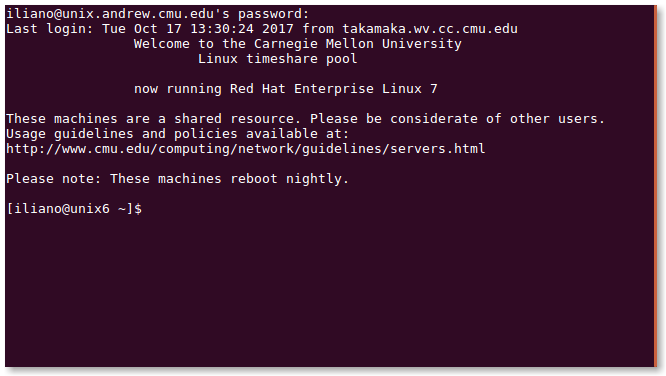
\includegraphics[width=0.75\linewidth]{\img/andrew-terminal.png}
\end{center}
\vspace{-2ex}
(The messages will look different for you.)


\newpage
\section*{Navigating your account in Linux}

\emph{Linux} is an operating system, just like Windows or Mac OS
X\@. If you want to know a little more about what's going on here,
look for the \qatool{} post titled ``What is Linux?''.

In this lab, rather than using a graphical interface,
you will use the terminal to enter commands directly to the OS\@.

\begin{part}\TAGS{unix}
    At the prompt, \textbf{\color{red}l}i\textbf{\color{red}s}t the
    files in your home directory\footnote{You're probably familiar
    with ``folders'' if you've used Mac or Windows. ``Directory''
    is the Linux name for
    folders.}
 by typing
\begin{lstlisting}[language={[coin]C}, belowskip=-1ex]
% ls
\end{lstlisting}
\end{part}

We often use the \lstinline[language={[coin]C}]'%'
or \lstinline[language={[coin]C},mathescape=false]'$' % $ (syntax highlighter confounder)
character at the
beginning of a line to indicate that it's something you're supposed to
enter at the prompt. Don't actually type it in! Just type
``\underline{\lstinline[language={[coin]C}]|ls|}'' and press Enter, don't type
``\lstinline[language={[coin]C}]|% ls|'' and then press Enter.

\begin{part}\TAGS{unix}
  You should see the directory \lstinline[language=]'private'
  as one of the entries in your home directory.  Move to this
  directory using the \underline{\lstinline[language={[coin]C}]'cd'}
    command, which lets you \textbf{\color{red}c}hange the \textbf{\color{red}d}irectory
    your terminal is working in.
\begin{lstlisting}[language={[coin]C}, belowskip=-1ex]
% cd private
\end{lstlisting}
\end{part}

\textbf{\textcolor{red}{ACADEMIC INTEGRITY NOTE:} You should store
  your program files and other class solutions inside the
  \lstinline[language=]'private' directory (or a subdirectory inside
  this directory) since this directory is automatically set to prevent
  electronic access by other users. Remember that you should protect
  your work from being accessed by other students as part of the
  academic integrity policy for this course.}


\begin{part}\TAGS{unix}
  Once you
  \underline{\lstinline[language={[coin]C}]'cd'} into the
    \lstinline[language=]'private' directory,
    \textbf{\color{red}m}a\textbf{\color{red}k}e a new
  \textbf{\color{red}dir}ectory named \lstinline[language=]'15122' using the
  \underline{\lstinline[language={[coin]C}]'mkdir'} command:
\begin{lstlisting}[language={[coin]C}]
% mkdir 15122
\end{lstlisting}
Now go into this directory using
  \underline{\lstinline[language={[coin]C}]'cd'} again:
\begin{lstlisting}[language={[coin]C}]
% cd 15122
\end{lstlisting}
\end{part}


% \bigskip\hrule\bigskip

% Let's create a directory for this lab, 'lab01', and go to it:
% \begin{lstlisting}[language={[coin]C}, belowskip=-1ex]
% % mkdir lab01
% % cd lab01
% \end{lstlisting}

\begin{comment}
\begin{part}\TAGS{unix}
  Download the handout for this lab by firing up a browser (e.g.,
  Firefox), pointing it to \autolab{}
  (\href{\autolabURL}{\autolabURL}), going to ``Lab 1: setup'' (this
  may be where you got this writeup from) and clicking on ``Download
  handout''.  There is also a copy of the handout on \qatool{}.

\enlargethispage{5ex}
\begin{description}
\item[{\em If you are on a GHC cluster computer},] this will save the
  handout as the file \lstinline'handout-01.tgz' in the 'Downloads'
  directory under the directory Terminal started at (that's your
  \emph{home directory}).  This is a compressed archive consisting of
  several files.  You can retrieve them with the following command:
\begin{lstlisting}[language={[coin]C}]
% tar xfzv ~/Downloads/handout-01.tgz
handout/
handout/factorial.c0
\end{lstlisting}

\item[{\em If you are on your own laptop},] you will need to transfer
  the file \lstinline'handout-01.tgz' on andrew so that you can access
  it through your terminal.  \textbf{\em If your are on a Mac or a
    Linux laptop}, open a terminal,
  \underline{\lstinline[language={[coin]C}]'cd'} to the directory
  where your browser saved \lstinline'handout-01.tgz' and run the
  command
\begin{lstlisting}[language={[coin]C}]
% scp handout-01.tgz <your_id>@unix.andrew.cmu.edu:private/15122/lab01
\end{lstlisting}
  It will ask for your andrew password.  Once you enter it, it will
  transfer the file to andrew.  You can check by running
  \underline{\lstinline[language={[coin]C}]'ls'} on your andrew
  terminal: it should be there!  You can uncompress this file by
  running
\begin{lstlisting}[language={[coin]C}]
% tar xfzv handout-01.tgz
handout/
handout/factorial.c0
\end{lstlisting}
If this command fails, try \lstinline'tar xfv handout-01.tgz' (without
the \lstinline'z').

\textbf{\em If you are on Windows}, you can transfer the
\lstinline'handout-01.tgz' interactively using one of the icons on
MobaXterm.  Ask a TA if you can't figure it out.  Then, proceed as
above.
\end{description}

This creates a directory called \lstinline'handout' containing the
  file \lstinline'factorial.c0'.  Go to this directory:

  \lstinline[language={[coin]C}]'% cd handout'
\end{part}

\begin{part}\TAGS{unix}
  Verify you are in the \lstinline[language={[coin]C}]'lab01/handout'
  directory by entering the command
  \underline{\lstinline[language={[coin]C}]'pwd'} to get the present
  working directory and by entering the command
  \underline{\lstinline[language={[coin]C}]'ls'} to see the files in that
  directory.  You should see something like this with your andrew id
  instead of \lstinline[language={[coin]C}]'<your_id>':

\begin{lstlisting}[language={[coin]C}]
% pwd
/afs/andrew.cmu.edu/<usr_number>/<your_id>/private/15122/lab01/handout
% ls
factorial.c0
\end{lstlisting}
\end{part}

\end{comment}
